\documentclass[letterpaper, 11pt]{Proposal}
\title{Assignment 1}
\author{Marcel Pascal Stolin}
\date{12th April 2022}

\def\Sec#1{Section~\ref{#1}}
\def\Fig#1{Figure~\ref{#1}}

\begin{document}

\vspace{-10cm}

\begin{textblock}{10}(3,1)
\textit{University of Trento}\\
\textit{Department of Computer Science}\\
\textit{Autonomous Software Agents}
\end{textblock}

\maketitle

\begin{tikzpicture}[overlay, remember picture]
  \node[xshift=-6cm,yshift=-1.6cm] at (current page.north east) {
\includegraphics[width=4.5cm,height=1.5cm]{logo_unitn}};
\end{tikzpicture}

\begin{tikzpicture}[overlay, remember picture]
  \node[xshift=-9.9cm,yshift=-3.6cm] at (current page.north east) {\includegraphics[width=1cm,height=1cm]{logo}};
\end{tikzpicture}

\vspace{-2cm}

% ===========================================
% ===========================================
\section{Introduction}\label{sec:01_intro}
% Why
Physical and psychological health does significantly benefit from good sleep.
What mostly affects sleep, is light.
It controls the body's internal clock when to sleep, 
regulates the circadian rhythm, 
and additionally influences the production of melatonin, 
a sleep-promoting hormone.

% The problem
However, in modern times, it is possible to provide 24/7
artificial illumination to brighten homes.
When people are exposed to artificial light most of the day, especially in the evening,
it negatively affects the quality of sleep \cite{SuniSleep2022}.

% Project goal
This project's goal is to provide a multi-agent solution,
that can control the lights in the house autonomously
in a way, that will increase the quality of sleep of the
residents and promote concentrating tasks during the day.

% Light sources
The sources of light in a standard house are light bulbs, 
and light that comes from the outside through the windows (sunlight and moonlight).

% Goals
The multi-agent is responsible for regulating the lightning in a room, 
by controlling the light bulbs of a room 
and eliminating the influence of the outside light.
When transitioning from day to evening, warm color temperatures 
and low illuminance help the human to relax.
At night, the bedroom needs to be as dark as possible to promote
the best possible quality of sleep, therefore all sources of light
need to be shut down.
Additionally, the electrically powered lights in a room are supposed to
be off, if no resident is present.

% ===========================================
% ===========================================
\section{Metrics}\label{sec:02_metrics}
% Light
Light is measured in lux, lumen, and wavelength and
all three influence the quality of sleep.
In this project, we are not interested in the wavelength metric.
Lumen is a measurement of brightness, and lux is a metric,
that measures the impact on the light to the surrounding space (illuminance).
As an example, a light bulb has a specific value of lumen, 
but the brightness of this bulb in the room is lux.

% Color temperature
In addition, a color is associated with a certain range of temperature, 
which is measured using the Kelvin scale.

\subsection{Illuminance}\label{subsec:02_metrics_illuminance}
% Overall
A clear day provides an illuminance of 10,000 lux outdoors.
In a room, this illuminance can break down to 25 - 50 lux. 
Therefore, artificial indoor lightning is still required during the day.

% During the day - Specific tasks
What level of lux to provide during the day, depends on the tasks done
by the residents in that room.
Overall, an illuminance level of 300 to 500 lux during the day is reasonable,
if no task, that requires concentration, is performed in that room.
For basic tasks like reading, a value of 500 - 800 lux is required.
Tasks that require high concentration require a higher illuminance of 800 - 1,700 lux.

% During the night
When it comes to the evening and the residents are transitioning from evening to bedtime,
an overall illuminance of 100 - 200 lux should be present.

% Sleep
When the residents start to sleep, all lightning devices are supposed to be off, 
and the windows need to be closed so that no outside light can come in.

% Difference adults childs
It is important to mention, that the lux level differs between adults and children.
However, no children are involved, therefore the values are based on adults \cite{SleepscoreLightAndTemp2022, AdamsLight2022}.

\subsection{Color Temperature}\label{subsec:02_metrics_temp}
% Commons
The following common color temperatures  \cite{EspositoTemp2022}:
\begin{itemize}
    \item Candlelight (lower than 2000K)
    \item Incandescent light (2000K - 3000K)
    \item Neutral light (3000K - 3500K)
    \item Cool white light (3600K - 4500K)
    \item Bright white light (4600K - 6500K)
    \item Clear sunlight (greater than 6500K)
\end{itemize}

% Morning and evening
In the morning and evening, a yellow color in the range of 2000K - 2700K
(Incandescent light) should be present.
% Bedtime
Before going to bed, an ideal temperature is 1900k (candlelight.)

% During the day
During the day, to increase productivity, a cool white in the range of 4000K - 6000k 
(Cool white light or bright white light) should be set \cite{BestTemp2022}.

% ===========================================
% ===========================================
\section{Devices}\label{sec:03_devices}
% What
This section provides details of the devices used in this scenario.

\subsection{Lights}\label{subsec:03_devices_lights}
% What
Lights provide artificial illuminations to the ambient light of the room.
% Technical specifications
Each single light bulb is a LED bulb and has a rated power consumption 
of 8.5W when powered on, and consumes a minimum of 0.5W on standby. 
It provides a range of 16 million different colors and the color temperature 
can be adjusted between 1700K-6500K.
Additionally, it provides 800 lumens.
% Other
The light bulb can only be fully turned off when disconnecting from the power source.

% Reference
\begin{figure}
    \centering
    \scalebox{0.5}{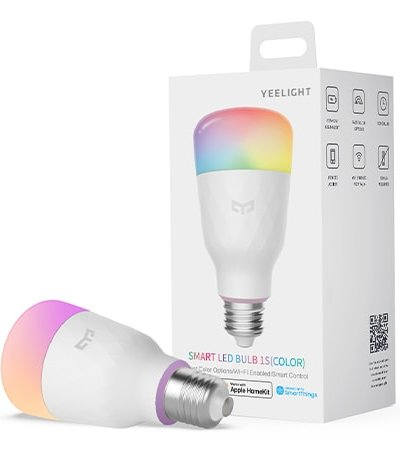
\includegraphics{img/yeelight-light-bulb-1s.jpeg}}
    \caption{Yeelight Smart LED Light Bulb 1S (Color)}
    \label{fig:03_devices_lights_yeelight}
\end{figure}
The reference model of a light bulb for this project is the 
\textit{Yeelight Smart LED Light Bulb 1S}\footnote{\url{https://us.yeelight.com/shop/yeelight-smart-led-light-bulb-1s-color/} (Accessed: 07-04-2022)}, 
as shown in \Fig{fig:03_devices_lights_yeelight}.

\subsubsection{States}
\begin{itemize}
    \item \texttt{ON} --- The light bulb is connected to electricity and connected 
    to the agent.
    \item \texttt{OFF} --- The light bulb is not connected to electricity.
    \item \texttt{STANDBY} --- The light bulb is connected to electricity but 
    does not provide light.
    \item \texttt{DISCONNECTED} --- The light bulb is connected to a power source 
    but not connected to the agent.
\end{itemize}

\subsubsection{Actions}
\begin{itemize}
    \item \texttt{TURN\_ON} --- Turn the device on, and connect to the agent.
    \item \texttt{TURN\_OFF} --- Turn the light bulb into a \texttt{STANDBY} state.
    \item \texttt{SET\_BRIGHTNESS} --- Set the brightness in lumens of the light bulb.
    \item \texttt{SET\_TEMP} --- Set the temperature in kelvin of the light bulb.
\end{itemize}

\subsection{Shutters}\label{subsec:03_devices_shutters}
% What
Shutters are used to preventing sunlight from going into the rooms.
They are attached to the outside of each window and can be closed using a 
built-in motor.
% How
A shutter can be closed by rolling the shutter down from the top of the 
window to the bottom.

% Figure
\begin{figure}
    \centering
    \scalebox{0.5}{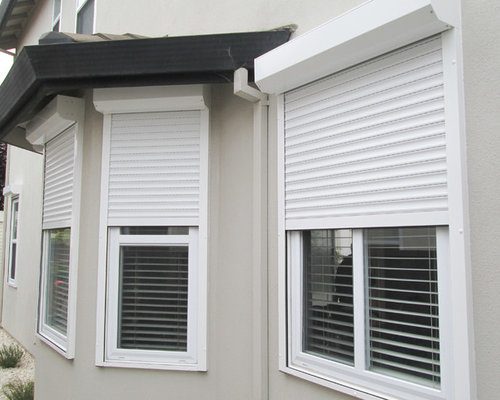
\includegraphics{rolling-shutter.jpeg}}
    \caption{A rolling exterior shutter on the outside of a window}
    \label{fig:03_devices_shutters_ref}
\end{figure}
% Reference
\Fig{fig:03_devices_shutters_ref} shows an example of an exterior rolling shutter, 
that is used in the scenario in this project.

\subsubsection{States}
\begin{itemize}
    \item \texttt{CONNECTED} --- The shutter is powered on and connected to the agent.
    \item \texttt{DISCONNECTED} --- The shutter is powered on, but not connected to the agent.
    \item \texttt{OFF} --- The shutter is not connected to a power source.
\end{itemize}

\subsubsection{Actions}
\begin{itemize}
    \item \texttt{TURN\_DOWN} --- Turn the shutter down.
    \item \texttt{TURN\_UP} --- Turn the shutter up.
\end{itemize}

\subsection{Motion Sensor}\label{subsec:03_devices_motion}
% What
The motion sensor triggers when a person enters a room.
Additionally, the motion sensor is able to detect if no person
is present in a room.

% Figure
\begin{figure}
    \centering
    \scalebox{0.3}{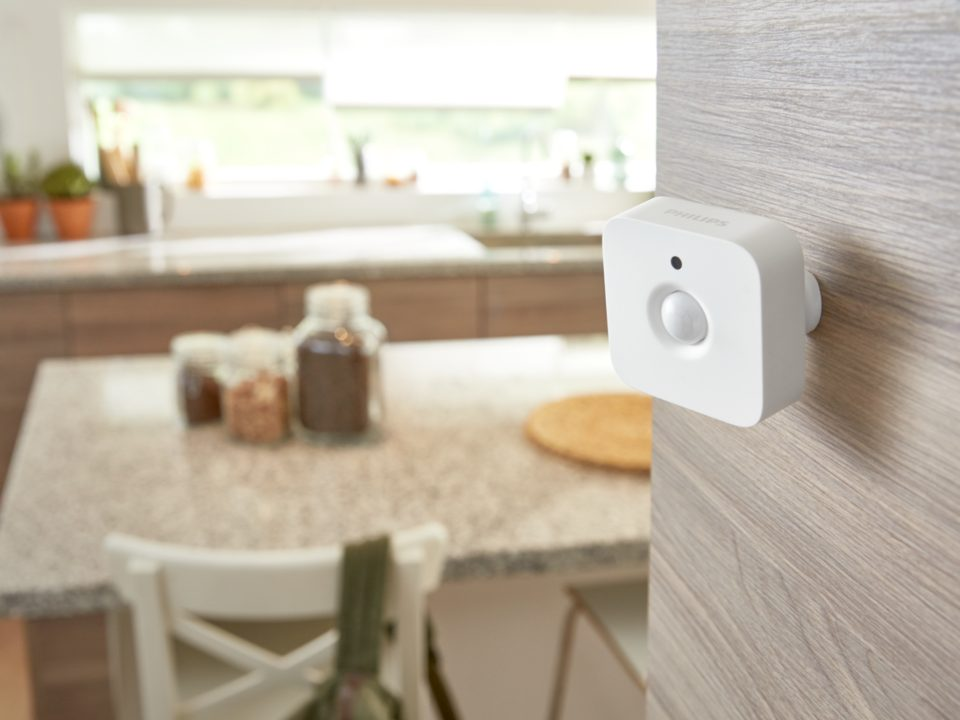
\includegraphics{motion_light_sensor.jpeg}}
    \caption{Philips Hue Motion Sensor, suitable as a light and motion sensor}
    \label{fig:03_devices_motion_ref}
\end{figure}
% References
A reference model for a motion sensor is the 
\textit{Philips Hue Motion Sensor}\footnote{\url{https://www.philips-hue.com/en-us/p/hue-motion-sensor/046677570972} (Accessed: 07-04-2022)}, 
as shown in \Fig{fig:03_devices_motion_ref}.
It is important to mention, that this device includes a motion and light sensor 
(for light sensor see section \Sec{subsec:03_devices_lightSensor}).
Using a 2in1 device is a good decision to save money and space 
and to reduce the setup complexity. However, in this project, both sensors are
threatened as a single device.

\subsubsection{States}
\begin{itemize}
    \item \texttt{ON} --- The motion sensor is powered on and connected to the agent.
    \item \texttt{OFF} --- The motion sensor is not connected to a power source.
    \item \texttt{DISCONNECTED} --- The motion sensor is powered on, but not connected to the agent.
\end{itemize}

\subsubsection{Actions}
\begin{itemize}
    \item \texttt{NOTIFY} --- Notifies the agent that a person has entered/left the room.
\end{itemize}

\subsection{Light Sensor}\label{subsec:03_devices_lightSensor}
% What
The light sensor is a device, that observes and measures the ambient light of a 
room in lux.
When the illuminance of a room change, it notifies the corresponding 
light agent of that room.

% Reference models
Reference models can either be the \textit{Philips Hue Motion Sensor}(see \Sec{subsec:03_devices_motion} for details about this device) or the
\textit{Xiaomi Mi Light Detection Sensor Zigbee 3.0}\footnote{\url{https://xiaomi-mi.com/sockets-and-sensors/xiaomi-mi-light-detection-sensor-zigbee-30/} (Accessed: 07-04-2022)}.

\subsubsection{States}
\begin{itemize}
    \item \texttt{ON} --- The light sensor is powered on and connected to the agent.
    \item \texttt{OFF} --- The light sensor is not connected to a power source.
    \item \texttt{DISCONNECTED} --- The light sensor is powered on, but not connected to the agent.
\end{itemize}

\subsubsection{Actions}
\begin{itemize}
    \item \texttt{ILLUMINANCE\_CHANGED} --- Notify the specific agent, that the illuminance of the room has changed.
\end{itemize}

\subsection{Room Controller}
% What
The room controller is a device that provides the residents to control the profile
of a room.
% Profiles
Overall, the residents can choose between three different profiles:
\begin{itemize}
    \item No-concentration --- Lightning between 300 - 500 lux is sufficient.
    \item Low-concentration --- Lightning between 500 - 800 lux is sufficient.
    \item High-concentration --- Lightning between 800 - 1,700 lux is sufficient.
\end{itemize}
% Default
By default, the no-concentration profile is active.
% Phone
In addition to the physical device, which is located in each room, a resident can
also change the profile with a smartphone.

\subsubsection{States}
\begin{itemize}
    \item \texttt{ON} --- The room controller is powered on and connected to the agent.
    \item \texttt{OFF} --- The room controller is not connected to a power source.
    \item \texttt{DISCONNECTED} --- The room controller is powered on, but not connected to the agent.
\end{itemize}

\subsubsection{Actions}
\begin{itemize}
    \item \texttt{CHANGE\_PROFILE} --- Notify the specific agent that a resident changed the profile for the room.
\end{itemize}

% ===========================================
% ===========================================
\section{House Description and Blueprint}\label{sec:04_houseDesc}
% What 
This section describes the house of the scenario.
The house has two floors, which are described in this section in detail.
Each floor section provides a blueprint of the floor and a detailed
description of each room.

% General devices
It is important to mention, that all rooms do include a motion sensor 
(\Sec{subsec:03_devices_motion}), and a light sensor (\Sec{subsec:03_devices_lightSensor}) 
to observe the movement and illuminance in the room.

\subsection{First Floor}\label{subsec:04_rooms_frstFloor}
% What
\Fig{fig:04_rooms_frstFloor_blueprint} illustrates the blueprint of 
the first floor.
Additionally, the blueprint also shows the location of light devices in the room.
It can be entered through the main entrance in the south and has 3 rooms, 
the lower floor, the living room, and the kitchen.
% Figure
\begin{figure}
    \centering
    \scalebox{0.4}{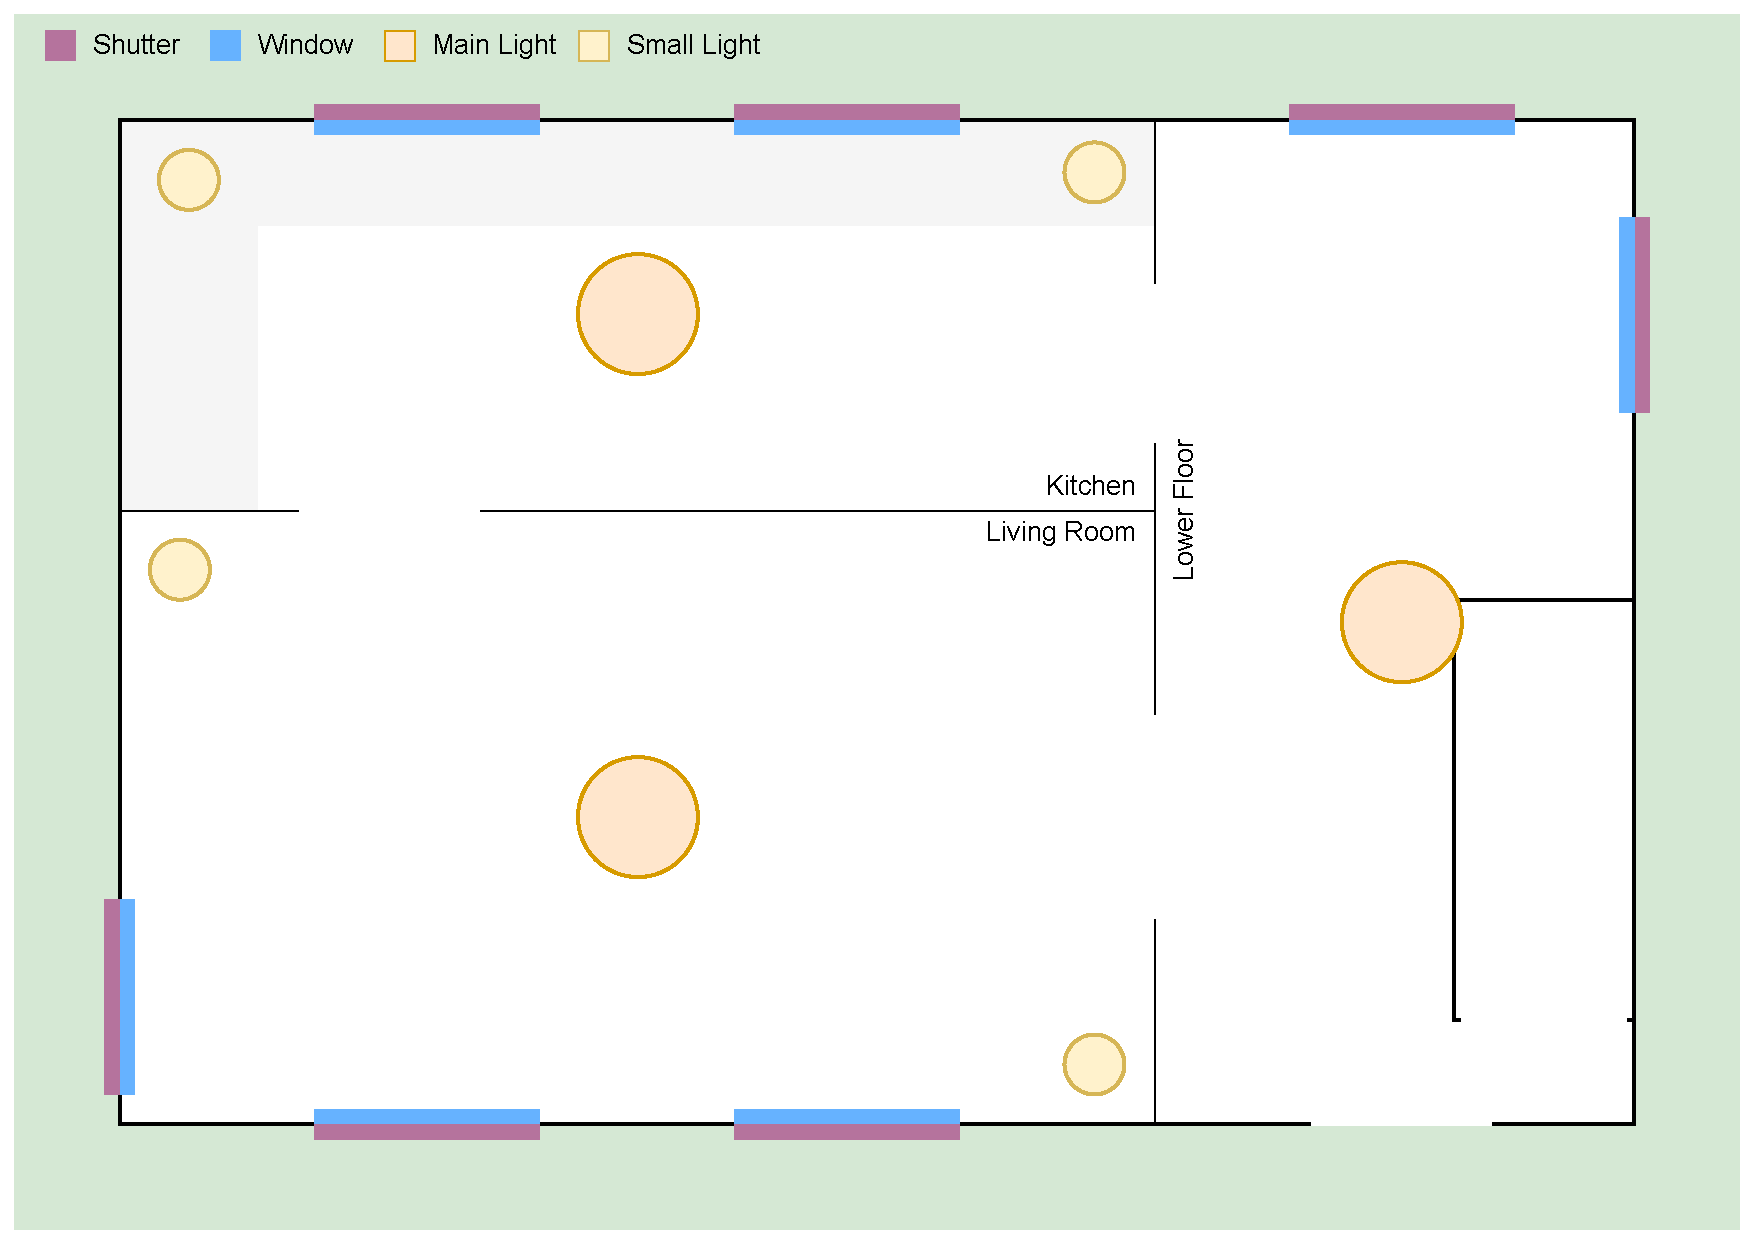
\includegraphics{img/blueprint_1st_floor.pdf}}
    \caption{First-floor blueprint}
    \label{fig:04_rooms_frstFloor_blueprint}
\end{figure}

\subsubsection{Lower Floor}\label{subsec:04_rooms_lowFloor}
% What
The lower floor on the first floor includes the main entrance to the house in the south.
Two additional doors in the west of the room, 
lead to the living room, or the kitchen.
Furthermore, the stairs to the second floor are located in this room.
Light is provided by a single main light on the ceiling in the middle of the room.
In addition, two windows, in the north, and one in the northeast are located
in the room.
% Usage
The only usage of this room is to get from one room to another or to 
get to the second floor. 
Therefore, no tasks requiring concentration are performed here.

\subsubsection{Living Room}\label{subsec:04_rooms_livRoom}
% What
Doors include the main entrance door in the east 
and the door to the kitchen in the north. 
Windows include two in the south and one in the west.
The living room has a main light in the middle of the room on the ceiling. 
Additional lights include two smaller lights in the north-west 
and southeast of the room.
% Usage
The living room is used by residents mostly in the morning and evening,
to eat breakfast or dinner, as well as to watch TV in the evening.
Therefore, only low concentration tasks, like reading or watching TV, 
are performed in this room.

\subsubsection{Kitchen}\label{subsec:04_rooms_kitchen}
% What
The kitchen includes two doors, one in the south and one in the east. 
The door in the south leads to the living room and the door in the east
leads to the lower floor.
It has a main light on the ceiling, as well as two lights in the work 
area of the kitchen, one in the northwest, and one in the northeast.
There are two windows in the north above the work area.
% Usage
The kitchen is used by residents to cook and prepare other foods/beverages. 
These tasks require high concentration.

\subsection{Second Floor}\label{subsec:04_rooms_scndFloor}
% What
The second floor is illustrated in \Fig{fig:04_rooms_scndFloor_blueprint}. 
It is reachable through the stairs from the first floor.
It includes the bedroom, a guest room, the bathroom, and the upper floor.
% Figure
\begin{figure}
    \centering
    \scalebox{0.4}{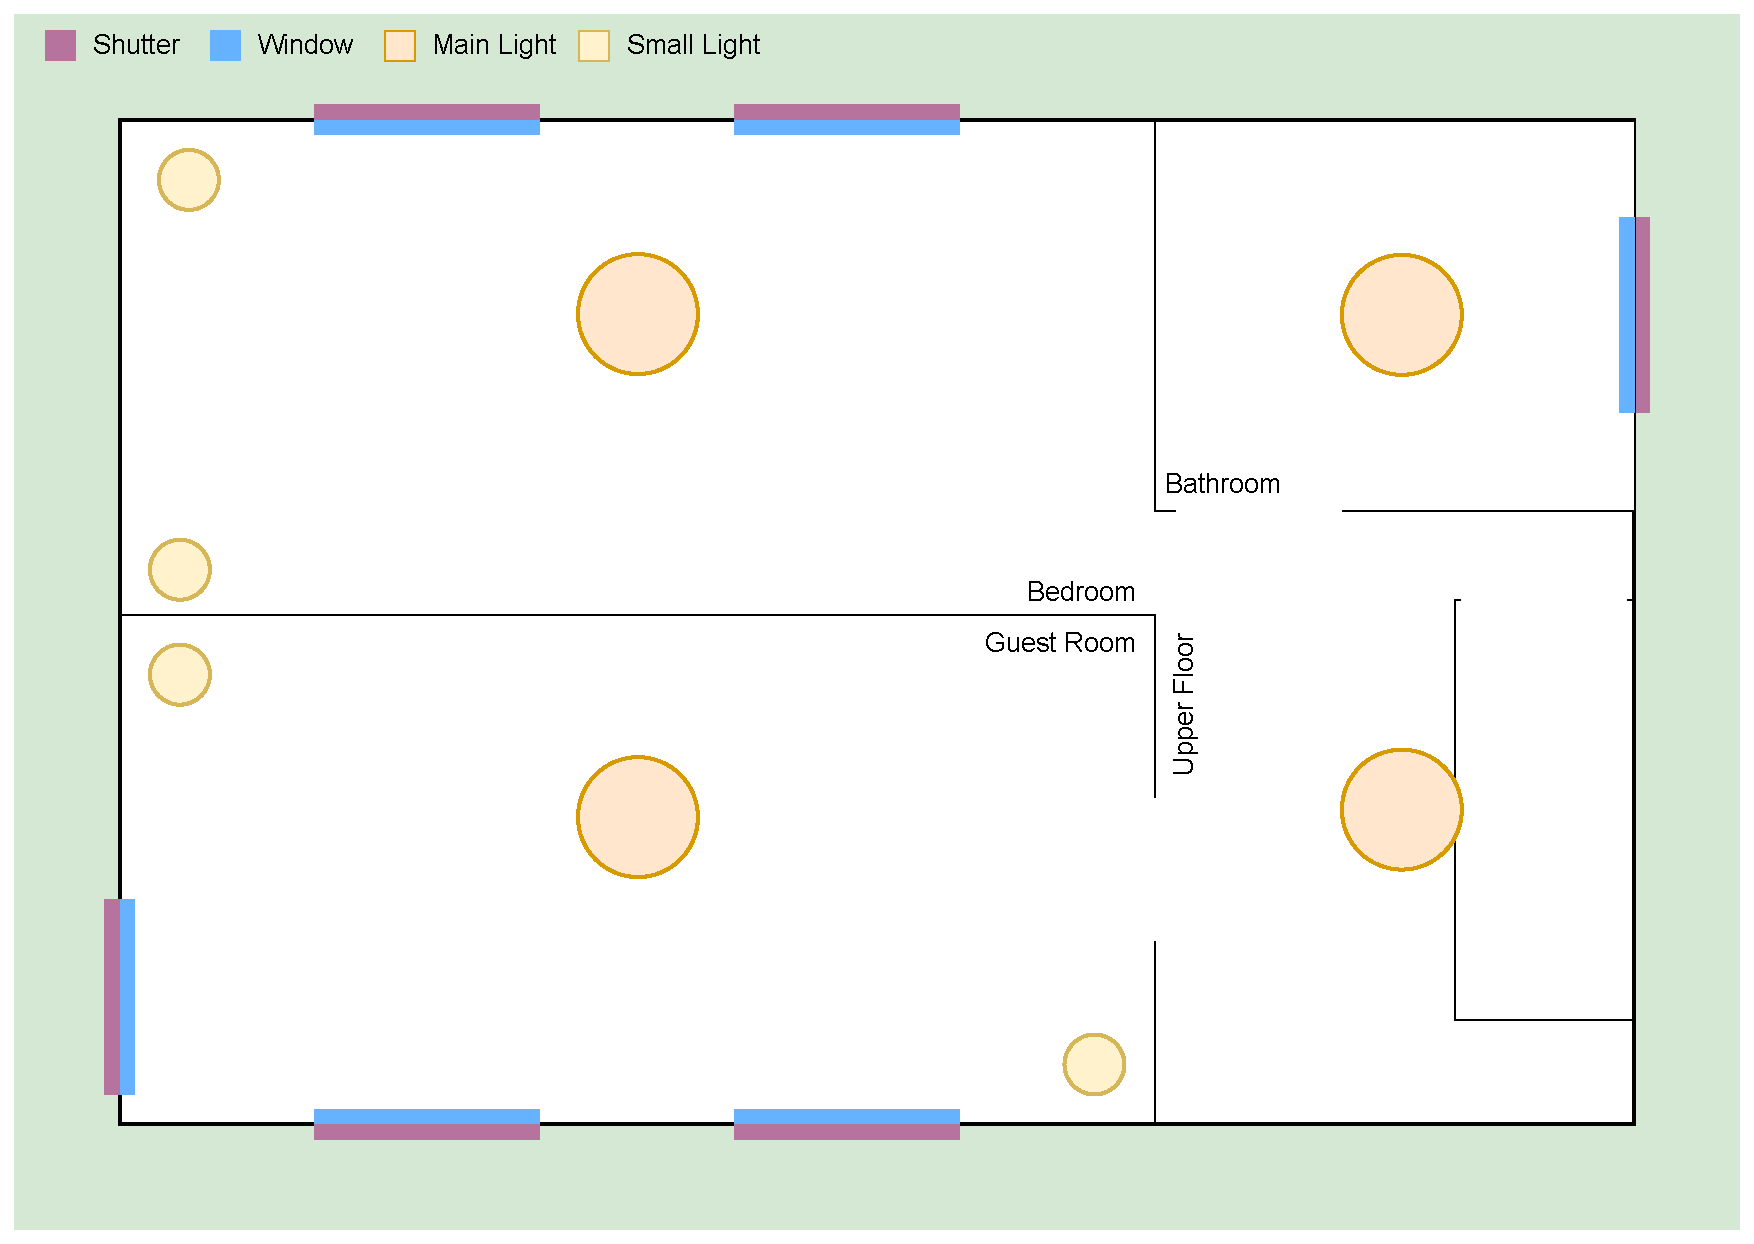
\includegraphics{img/blueprint_2nd_floor.pdf}}
    \caption{Second-floor blueprint}
    \label{fig:04_rooms_scndFloor_blueprint}
\end{figure}

\subsubsection{Upper Floor}\label{subsec:04_rooms_upFloor}
% What
The upper floor is the entrance to the second floor of the house.
It includes the stairs from the first floor.
Light is provided by a single main light on the ceiling.
Three doors are included in this room. 
One door in the north to the bathroom, and two doors
in the west, one to the guest room, and one to the bedroom.
No additional windows are included in this room.
% Usage
The upper floor is used like the lower floor. 
Therefore, concentration is not required in this room.

\subsubsection{Bedroom}\label{subsec:04_rooms_bedroom}
% What
This room includes one door in the east to the upper floor.
Two windows are located in the north of the room.
The main light is located in the middle of the room on the ceiling,
and two additional small lights are located in the northwest and southwest.
% How
The bedroom is used for sleeping, in the morning and in evening.
Sometimes, the residents like to read to relax during the day or in the evening,
which is a low-concentration task.

\subsubsection{Guestroom}\label{subsec:04_rooms_guestroom}
% What
The guest room includes one door to the floor in the east.
Windows include two in the south and one in the west.
It has one main light on the ceiling, two small lights in the northwest 
and one in the southeast.
In addition, it includes a desk with a computer.
% Usage
The room is mostly used either for guest sleepovers or for working.
Working is a high-concentration task.

\subsubsection{Bathroom}\label{subsec:04_rooms_bathroom}
% What
The bathroom has a single door in the south of the room
which leads to the upper floor.
A single main light on the ceiling is provided in the middle
of the room.
One window is located in the east.
% Usage
Residents use the bathroom for their hygiene. This requires either
high- or low-concentration light.

% ===========================================
% ===========================================
\section{Agents}\label{sec:05_agents}
% What
This section describes the agents in the multi-agent scenario, that is
responsible to provide the autonomous behavior.

\subsection{House Agent}
% What
The house agent is responsible to assist the device-specific agents of
the multi-agent environment.
% Movements
It connects to the motion sensors (\Sec{subsec:03_devices_motion}) of each room 
and can detect the resident's movements.
% Detect daytimes
Additionally, the house agent is aware of the geographical location of
the house, can differentiate between different daytimes 
(morning, afternoon, evening, bedtime), and knows about the time of sunrise and sunset.
% Shutters
According to the daytime, the house agents open or close the window shutters.

% Procedures and events
The following are common procedures and events, the house is responsible for:
\begin{itemize}
\item Observe the movement of the residents in the house.
\item When a resident enters/leaves a specific room, notify the corresponding light agent of the room.
\item Notify the light agents, when the daytime has changed. 
\item Open the window shutter during sunrise, and close the window shutter during sunset.
\end{itemize}

\subsection{Light Agent}
% What
A light agent is a device-specific agent and controls the lightning devices 
(light bulbs, see \Sec{subsec:03_devices_lights}) of a specific room. 
% How
It is assisted by the house agent, and responsible to adjust the ambient light of a room
in accordance with the daytime, if a resident is present.
Overall, it is responsible to create an environment in a room, where the residents
can either relax before bedtime or do concentrating tasks.
% Illuminance
To get information about the illuminance of a room, it can communicate with the
light sensor of its room.

% Procedures and events
The following are the specific procedures and events, the light agent is responsible for:
\begin{itemize}
    \item Turn light devices on/off when a resident enters/leaves the room.
    \item Decide which devices are not needed, to fulfill the desired state 
    (e.g.: Prefer main light over small lights during the day).
    \item Adjust the illuminance and color temperature of a room 
    (see \Sec{sec:02_metrics}), according to the daytime.
\end{itemize}

% ===========================================
% ===========================================
\section{People}\label{sec:06_people}
The residents of the house are the couple Sandra and Bob. 
Both can be in one room at a time, 
in two different rooms, or out of the home. 
Sandra works during the workdays from 08:00 to 17:00 Monday - Friday. 
Bob works from home while being self-employed, 
he has no specific work time. 
However, he does not work after 18:00.
On the weekend, they both are either at home or outside. 
Usually, on all days, in the evening they like to watch TV 
from 19:00 to 21:00 and go to sleep at 22:00.
Between 21:00 and 22:00, both residents like to read in the bed.

\bibliographystyle{IEEEtran}
\bibliography{bibliography}

\end{document}
